% Copyright (c) 2015 Benito Palacios Sánchez - All Rights Reserved.
% Esta obra está licenciada bajo la Licencia Creative Commons Atribución 4.0
% Internacional. Para ver una copia de esta licencia, visita
% http://creativecommons.org/licenses/by/4.0/.

% Template
\documentclass{beamer}

% Notes. Uncomment to view the notes.
%\setbeameroption{show notes}
%\setbeamertemplate{note page}[plain]    % Remove the note page style

% Font
\usepackage[T1]{fontenc}                % Output font
\usepackage[utf8]{inputenc}             % Input encoding
\usepackage[spanish,es-tabla]{babel}    % For Spanish texts
\usepackage{FiraSans}

% Theme
\usetheme{Darmstadt}
\usecolortheme{whale}

% Other packages
\usepackage{url}                % For links
\usepackage{graphicx}           % For graphics
\usepackage{verbatim}           % For non-parsed text blocks
\usepackage{listings}           % For blocks of code
\lstset{language=[Sharp]C,basicstyle=\scriptsize\ttfamily,                 keywordstyle=\scriptsize\color{blue}\ttfamily}

% My package
\usepackage{Layout}

% Information about author and document
\title{Mecanismos de protección de datos en videojuegos}
\date[Julio de 2015]{15 de julio de 2015}
\author{Benito Palacios}
\institute[UGR]
{Escuela Técnica Superior de Ingenierías Informática y Telecomunicación (UGR)}
\university{Universidad de Granada}
\departament{Dpto. Teoría de la Señal, Telemática y Comunicaciones}
\titlelogo{imgs/ugr_logo.pdf}
\tutor{Dr.~D. Pedro García Teodoro}

% Add a little logo in the corner of the slides
\pgfdeclareimage[height=0.5cm]{university-logo}{imgs/ugr_logo_mini.pdf}
\logo{\pgfuseimage{university-logo}}

\begin{document}

    % Copyright (c) 2015 Benito Palacios S�nchez - All Rights Reserved.
% Esta obra est� licenciada bajo la Licencia Creative Commons Atribuci�n 4.0
% Internacional. Para ver una copia de esta licencia, visita
% http://creativecommons.org/licenses/by/4.0/.

\chapter{Introducci�n}

    % Copyright (c) 2015 Benito Palacios Sánchez - All Rights Reserved.
% Esta obra está licenciada bajo la Licencia Creative Commons Atribución 4.0
% Internacional. Para ver una copia de esta licencia, visita
% http://creativecommons.org/licenses/by/4.0/.

\section{Introducción}
\subsection{}

\begin{frame}{Motivación}
\begin{columns}
    \begin{column}{0.5\textwidth}
    \begin{wideitemize}
        \item<1-> Los videojuegos son una clave de nuestra cultura actual.

        \item<2-> Su industria es la segunda con más ganancias.

        \item<3-> Preocupación por protección anti-copias, derechos de autor, trampas.
    \end{wideitemize}
    \end{column}

    \begin{column}{0.5\textwidth}
        \only<1>{
            \includefigure{Estadísticas sobre jugadores en EE. UU. \scriptsize{}Fuente: \url{http://www.esrb.org} (2010).}{imgs/gamer_stats.png}
        }

        \only<2->{
            \includefigure{Estadísticas sobre la industria de videojuegos en EE. UU. \scriptsize{}Fuente: \url{http://www.esrb.org} (2009).}{imgs/game_ind_stats.png}
        }
    \end{column}
\end{columns}
\end{frame}

\begin{frame}{\textit{ROM Hacking}}
    \begin{block}{Ingeniería inversa}
        La ingeniería inversa es el proceso de analizar un sistema para identificar sus componentes y relaciones y, crear una representación del sistema en otro formato o a un nivel más alto de abstracción.
    \end{block}

    \begin{block}{\textit{ROM Hacking}}<2->
        Ingeniería inversa sobre videojuegos. El nombre viene realizar modificaciones (\textit{hacks}) sobre juegos que suelen distribuirse en memorias de solo lectura (\textit{Read Only Memory}).
    \end{block}
\end{frame}


    % Copyright (c) 2015 Benito Palacios Sánchez - All Rights Reserved.
% Esta obra está licenciada bajo la Licencia Creative Commons Atribución 4.0
% Internacional. Para ver una copia de esta licencia, visita
% http://creativecommons.org/licenses/by/4.0/.

\section[Fan-traducciones]{Traducciones no oficiales}
\subsection{Saga Pokémon}
\begin{frame}{Saga Pokémon}

\end{frame}

\begin{frame}{Metodología}
\end{frame}

\begin{frame}{Pokémon Perla y Diamante}

\end{frame}

\begin{frame}{Pokémon HeartGold y SoulSilver}

\end{frame}

\begin{frame}{Pokémon Blanco y Negro}

\end{frame}

\begin{frame}{Pokémon Conquest}

\end{frame}

\subsection{Ninokuni: El Mago de las Tinieblas}
\begin{frame}{Ninokuni: El Mago de las Tinieblas}

\end{frame}

    % Copyright (c) 2015 Benito Palacios Sánchez - All Rights Reserved.
% Esta obra está licenciada bajo la Licencia Creative Commons Atribución 4.0
% Internacional. Para ver una copia de esta licencia, visita
% http://creativecommons.org/licenses/by/4.0/.

\section[Contenido con copyright]{Contenido con derechos de autor}
\subsection{Libros electrónicos}
\begin{frame}{Ninokuni}

\end{frame}

\begin{frame}{100 Classic Book Collection}

\end{frame}

\subsection{Bandas sonoras}
\begin{frame}{Guitar Hero: On Tour}

\end{frame}

\begin{frame}{Duet}

\end{frame}

    % Copyright (c) 2015 Benito Palacios Sánchez - All Rights Reserved.
% Esta obra está licenciada bajo la Licencia Creative Commons Atribución 4.0
% Internacional. Para ver una copia de esta licencia, visita
% http://creativecommons.org/licenses/by/4.0/.

\section{Servicios en línea}
\subsection{Multijugador}
\begin{frame}[fragile]{Captura de paquetes}
\begin{columns}

\begin{column}{0.35\textwidth}
Estrategia \textit{man-in-the-middle}
\begin{center}
    \includefigure{\textit{Man-in-the-middle}}{imgs/man_middle.eps}
\end{center}
\end{column}

\begin{column}{0.5\textwidth}
\uncover<2->{Modificación DeSmuME.}
\begin{itemize}
    \item<3-> Paquetes PCAP.
\end{itemize}
\begin{uncoverenv}<3->\begin{lstlisting}
void create_packet();
void save_packet(u8* packet,u32 len);
void save_adhocPacket(u8* packet,
  u32 len, void* addr, bool isSent);
\end{lstlisting}\end{uncoverenv}

\begin{itemize}
    \item<4-> Exportar paquetes.
\end{itemize}
\uncover<5->{\scriptsize\texttt{HandleDebugEvent\_Execute()} en \texttt{debug.cpp}.}
\vfill
\visible<6->{\includefigure{\textit{RC4Finder.}}{imgs/rc4finder.png}}
\end{column}

\end{columns}
\end{frame}

\begin{frame}{Servidores para Nintendo DS}

\begin{center}
    \visible<2->{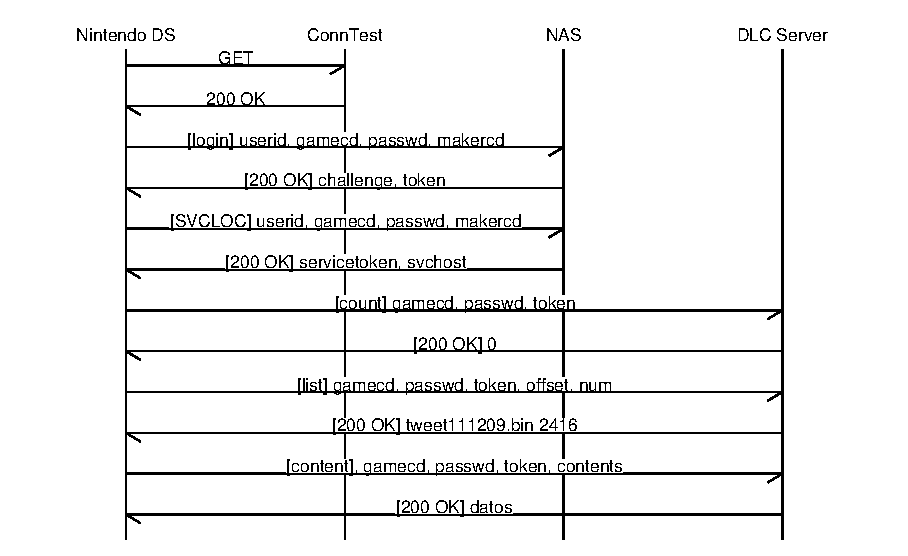
\includegraphics[width=\textwidth,height=0.5\textheight,keepaspectratio]{imgs/nds_dwc.eps}}
\end{center}

\uncover<3->{Vulnerabilidades:}
\begin{columns}
\footnotesize
\begin{column}{0.3333\textwidth}
    \begin{itemize}
        \item<4-> Puerto 80 del NAS abierto.
    \end{itemize}
\end{column}
\begin{column}{0.3333\textwidth}
    \begin{itemize}
        \item<5-> Contraseña no usada.
    \end{itemize}
\end{column}
\begin{column}{0.3333\textwidth}
    \begin{itemize}
        \item<6-> Autenticación simple.
    \end{itemize}
\end{column}

\end{columns}
\end{frame}

\begin{frame}{Preguntados}
\begin{columns}
    \begin{column}{0.15\textwidth}
        
\includegraphics[width=\textwidth,keepaspectratio]{imgs/preguntados_logo.png}
    \end{column}
    \begin{column}{0.85\textwidth}
        Trivial para plataformas móviles.
    \end{column}
\end{columns}

\vfill
\vspace{0.35cm}
\uncover<2->{Vulnerabilidades:}
\begin{columns}
    \begin{column}{0.5\textwidth}
    \begin{itemize}
        \item<3-> Comunicación HTTP.
    \end{itemize}
    \end{column}

    \begin{column}{0.5\textwidth}
    \begin{itemize}
        \item<4-> Solución enviada antes de preguntar.
    \end{itemize}
    \end{column}
\end{columns}

\only<4>{\includefigure{Preguntas, respuesta y solución de una partida}{imgs/preguntados_hack.png}}

\only<5>{\includefigure{Preguntas, respuesta y solución de una partida}{imgs/preguntados_hack_question.png}}

\only<6>{\includefigure{Preguntas, respuesta y solución de una partida}{imgs/preguntados_hack_answer.png}}

\end{frame}

\subsection{Contenidos descargables}
\begin{frame}{Duet}
\begin{center}
\includegraphics[width=0.15\textwidth,keepaspectratio]{imgs/duet_logo.png}\end{center}

\begin{columns}
    \begin{column}{0.5\textwidth}
    \begin{itemize}
        \item<2-> Niveles extras por 0,99€.
        \item<4-> BD con preferencias sin proteger.
        \note<1>[item]{Es SQLite y se puede usar software como SQLiteMan}
    \end{itemize}
    \end{column}

    \begin{column}{0.5\textwidth}
    \begin{itemize}
        \item<3-> Ya incluídos pero desactivados.
        \item<5-> Se puede activar a mano.
    \end{itemize}
    \end{column}
\end{columns}

\visible<5->{\includefigure{Filas con estado de los contenidos extras}{imgs/duet-levels.png}}

\end{frame}

\begin{frame}{\textit{Download Play}}
Compartir demos con comunicación inalámbrica ad-hoc.
\vfill
\uncover<2->{\underline{Problema:}}
\begin{itemize}
    \item<3-> Envío de código de una consola a otra.
    \item<4-> El código principales se firman con \texttt{RSA}.
\end{itemize}
\vfill
\uncover<5->{\underline{Solución de Nintendo:}}
\begin{itemize}
    \item<6-> Comprobar integridad con \texttt{HMAC}.
    \item<7-> Solo si con \textit{Download Play}.
\end{itemize}
\end{frame}


    % Copyright (c) 2015 Benito Palacios Sánchez - All Rights Reserved.
% Esta obra está licenciada bajo la Licencia Creative Commons Atribución 4.0
% Internacional. Para ver una copia de esta licencia, visita
% http://creativecommons.org/licenses/by/4.0/.

\section{Conclusiones}
\subsection{}

\begin{frame}{Conclusiones}
Objetivos alcanzados:
\begin{wideitemize}
    \item<+-> Identificar problemas no tratados en la literatura.

    \item<+-> Desarrollar software.

    \item<+-> Aprender conceptos de bajo nivel en software y hardware incluyendo el lenguaje ensamblador \texttt{ARM}.

    \item<+-> Diseñar metodologías de ingeniería inversa y captura de paquetes.

    \item<+-> Analizar 21 juegos.

    \item<+-> Aprender \LaTeX.
\end{wideitemize}
\end{frame}

\begin{frame}{Trabajo futuro}
\begin{wideitemize}
    \item<+-> Estudios:
    \begin{itemize}
        \item<+-> Seguridad en videoconsolas y sus \textit{exploits}.
        \item<+-> Algoritmos de integridad en archivos de guardado.
        \item<+-> Mecanismos anti-copia físicos y digitales.
        \item<+-> Protocolos de micropagos en videojuegos.
        \item<+-> Seguridad de aplicaciones de ordenador (\textit{Steam}).
    \end{itemize}

    \item<+-> Desarrollos:
    \begin{itemize}
        \item<+-> Implementar mecanismos estudiados.
        \item<+-> Explorador de juevos avanzado.
        \item<+-> Depurador de código remoto.
    \end{itemize}
\end{wideitemize}
\end{frame}


    % Copyright (c) 2015 Benito Palacios Sánchez - All Rights Reserved.
% Esta obra está licenciada bajo la Licencia Creative Commons Atribución 4.0
% Internacional. Para ver una copia de esta licencia, visita
% http://creativecommons.org/licenses/by/4.0/.

\appendix
\section{\appendixname}
\frame{\tableofcontents}

\subsection{Metodología}
\begin{frame}

\end{frame}

\subsection{Traducciones no oficiales}
\begin{frame}{Pokémon HeartGold y SoulSilver}

\end{frame}

\begin{frame}{Pokémon Conquest}

\end{frame}

\begin{frame}{Ninokuni: El Mago de las Tinieblas}

\end{frame}

\subsection{Contenidos con derechos de autor}
\begin{frame}{100 Classic Book Collection}

\end{frame}


\subsection{Servicios en línea}
\begin{frame}{100 Classic Book Collection}

\end{frame}

\begin{frame}{Ninokuni: El Mago de las Tinieblas}

\end{frame}


\end{document}
